% Modelo Canônico de documento usando o abntlatex
\documentclass[oneside]{abntlatex}
\usepackage{graphicx}

% Uso de recursos de matemática
\usepackage{amsmath}
%\usepackage{amssymb} nao e necessario mais apos a versao atualizada do pacote MNRAS

% Recursos extras
\usepackage{steinmetz}  % usar números polares
\usepackage{subcaption} % usar subfigure
\usepackage{float}
\usepackage{lipsum}
\usepackage{xcolor}

% --- Configurações dos pacotes ---
% ---
\graphicspath{{./figures/}} % default Path

\makeatletter
\hypersetup{
  pdftitle = {\@title}, 
  pdfauthor = {\@author},
  pdfcreator = {LaTeX2e with ABNT},
  pdfkeywords = {latex }{ABNT }, 
  pdfpagemode = FullScreen,
  colorlinks = false,
  linkbordercolor = red,
  citebordercolor = red,
  urlbordercolor = red
}
\makeatother
% ---

\title        {Modelo canônico de artigo científico em \LaTeX usando abnt\LaTeX :}
\subtitle     {Análise de um circuito de um filtro passivo}
\university   {Universidade de NOME-DA-UNIVERSIDADE - SIGLA-DA-UNIVERSIDADE}
\author       {NOME-DO-AUTOR}
\predate      {LOCAL, LOCAL}
\date         {\the\year}
\documenttype {Exemplo de artigo científico.}
\preamble     {Artigo científico apresentado à disciplina de NOME-DA-DISCIPLINA para obter aprovação na disciplina SIGLA-DA-DISCIPLINA.}
\supervisor   {NOME-ORIENTADOR}
\cosupervisor {NOME-COORIENTADOR}
\keywords     {LaTeX, ABNT}

\begin{document}
  \pretext%
  % --- Parte externa (NBR 14724/2011) ---
  % ---
  \maketitle % Capa
  % Lombada (opcional)
  % ---

  % --- Elementos Pré-textuais (NBR 14724/2011) ---
  % ---
  \coverpage%       Folha de rosto                 (obrigatório)
  %                 Errata                         (opcional)
  %                 Folha de aprovação             (obrigatório)
  %                 Dedicatória                    (opcional)
  %                 Agradecimentos                 (opcional)
  %                 Epínagrefe                     (opcional)
  \begin{abstract}% Resumo na língua vernácula     (obrigatório)
    \lipsum[1-1]
  \end{abstract}
  %                 Resumo na língua estrangeira   (obrigatório) 
  \listoffigures%   Lista de ilustrações           (opcional)
  \listoftables%    Lista de tabelas               (opcional)
  %                 Lista de abreviaturas e siglas (opcional)
  %                 Lista de símbolos              (opcional)
  \tableofcontents% Sumário                        (obrigatório)
  % ---

  % --- Elementos Textuais ---
  % ---
  \maintext%

  % Seção 1. Introdução
  \section{Introdução}
  Para o documento de exemplo vai ser feita uma análise de um circuito de um filtro passivo de passa-baixas, composto por um resistor e um capacitor.

  Um filtro tem a capacidade de atenuar ou realçar a amplitude de um sinal para certas bandas de frequência do sinal, visando, por exemplo reduzir o ruído de sinais em determinado espectro, ou para resolver um grande problema nas transmissões de sinais em longa distância, já que ocorrem perdas do sinal em altas frequência, fazendo com
  que tenha uma incoerência do sinal no receptor e transmissão \cite{ref:all_about_audio}. Um filtro passivo é um filtro que não requer energia externa para operar, diferentemente dos filtros ativos, consistindo apenas de componentes passivos (indutores, capacitores e resistores). Sendo os principais filtros: passa-faixa, passa-altas e passa-baixas.

  Os filtros de passagem permitem passar apenas frequências abaixo, entre ou acima de
  um ponto de corte de frequência especificado, depende se o filtro é passa-baixas, passa-faixa ou passa-altas, respectivamente sendo possível remover certas frequências indesejadas, ou isolar uma banda no caso do passa-faixa.

  \subsection{Filtros de passagem}
    \subsubsection{Passa-baixas}
      O filtro passa-baixas (também conhecido com \textit{high cut}) é um tipo de circuito que faz com que a potência sonora em frequências a partir de uma determinada frequência especificada (chamada frequência de corte) seja reduzida à metade da potência original, ou seja, permitindo que apenas as frequências mais graves mantenham valores mais próximos de sua potência inicial.

    \subsubsection{Passa-altas}
      Com funcionamento bastante similar ao passa-baixas, o filtro passa-altas (também conhecido com \textit{low cut}) por sua vez tem a função de reduzir o ganho das frequências inferiores à uma determinada frequência de corte, permitindo que as frequências superiores à de corte mantenham uma potência mais parecida com a de origem.

    \subsubsection{Passa-faixa}
      O filtro passa-faixa tem como característica principal, permitir a passagem com
      ganho mais parecido ao do sinal original, frequências próximas à uma frequência definida (denominada frequência de ressonância), enquanto que frequências abaixo e acima de frequências especificadas (denominadas frequência de corte inferior e frequência de corte superior, respectivamente) sejam reduzidas em potência.

  % Seção 2. Análise teórica
  \section{Análise teórica do passa-baixas}
  Como apresentado previamente, os filtros passa-baixas tem como característica a capacidade de atenuar sinais com frequências grandes, acima de uma frequência linear de corte, $f_c$ ou frequência angular de corte, $\omega_c$, definidas. Uma topologia indicada para se utilizar é a de um circuito RC de resistor em série com um capacitor em que a saída de tensão do circuito ocorre sobre o capacitor.

  Considerando o circuito RC série com a saída sobre o capacitor, $v_{out}$, dado na figura \ref{fig:esquematico_passa_baixas}, em regime permanente senoidal (RPS), alimentado por um gerador ideal senoidal, $v_{in}$.

  \begin{figure}[H]
    \centering
    \caption{Esquemático de um circuito passa-baixas}
    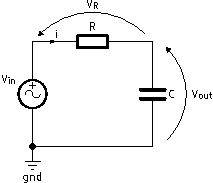
\includegraphics[width = 0.6 \linewidth]{passa-baixas.pdf}
    \fontfigure{Elaboração Própria (Kicad)(\the\year)}
    \label{fig:esquematico_passa_baixas}
  \end{figure}

  É possível obter as equações e os gráficos do módulo e fase da resposta em frequência do circuito considerando a impedância dos componentes como $R$ e $\frac{1}{j \omega C}$, resistor e capacitor, respectivamente, as tensões dadas em fasores como $\hat{v}_{in}$, $\hat{v}_{R}$ e $\hat{v}_{out}"$, sendo as tensões sobre a fonte, o resistor e o capacitor, respectivamente e a corrente do circuito dada como $\hat{i}$.

  Utilizando as relações constitutivas dos bipolos dados temos que:

  \begin{equation*}
    \begin{cases}
      \hat{v}_{out} = \frac{1}{j \omega C} \cdot \hat{i} \\
      \hat{v}_{R} = R \cdot \hat{i}
    \end{cases}
  \end{equation*}

  Pela segunda lei de Kirchhoff (\textit{Kirchhoff's Voltage Law}), tem-se:

  \begin{equation} 
    \mathbf{KVL:} \quad \hat{v}_{in} = \hat{v}_{R} + \hat{v}_{out} = R \cdot \hat{i} + \hat{v}_{out}
    \label{eq:kvl_passa_baixas}
  \end{equation}

  Analisando o circuito, considerando-o com apenas um bipolo de impedância total $Z$, pode-se obter a corrente do circuito isolando-a na equação:

  \begin{equation}
    \hat{v}_{in} = Z \cdot \hat{i} = \left( R + \frac{1}{j \omega C} \right) \cdot \hat{i} \Rightarrow \hat{i} = \frac{\hat{v}_{in}}{R + \frac{1}{j \omega C}}
    \label{eq:corrente_passa_baixas}
  \end{equation}

  Com isso, substituindo a equação \ref{eq:corrente_passa_baixas} na \ref{eq:kvl_passa_baixas} é possível obter a expressão da resposta em frequência dada por $G(j \omega)$.

  \begin{equation*}
    \sp{(\ref{eq:corrente_passa_baixas}) \rightarrow (\ref{eq:kvl_passa_baixas})}
    \quad \hat{v}_{in} = R \cdot \frac{\hat{v}_{in}}{R + \frac{1}{j \omega C}} + \hat{v}_{out} \Rightarrow \frac{\hat{v}_{out}}{\hat{v}_{in}} = 1 - \frac{R}{R + \frac{1}{j \omega C}} = \frac{1}{1 + j \omega R C} = G(j \omega) 
  \end{equation*}

  \begin{equation}
    \therefore \quad G(j \omega) = \frac{1}{\sqrt{1 + \left(\omega R C\right)^2}} \phase{-\arctan(\omega R C)}
    \label{eq:ganho_passa_baixas}
  \end{equation}

  A partir da expressão, \ref{eq:ganho_passa_baixas}, obtida é possível construir os gráficos, apresentados na figura \ref{fig:grafico_passa_baixas}, que apresentam o valor em módulo e da fase de $G(j\omega)$ em função da frequência angular, $\omega$, analisando os gráficos é possível reconhecer e calcular pontos importantes da curva, como os pontos para que $|G(j0)| = 1$ para $\omega = 0$, que $ \lim_{\omega\to\infty} |G(j\omega)| = 0$ e $|G(j \omega)| = \frac{1}{\sqrt{2}}$, para $\omega = \frac{1}{RC}$, que indica o momento em que a potência média de saída cai pela metade de seu valor máximo, sendo o momento onde ocorre a frequência de corte, logo $\omega_c = \frac{1}{RC}$.

  \begin{figure}[H]
    \centering
    \caption{Gráficos do circuito passa-baixas, módulo e fase, respectivamente}
    \begin{subfigure}{0.5 \linewidth}
      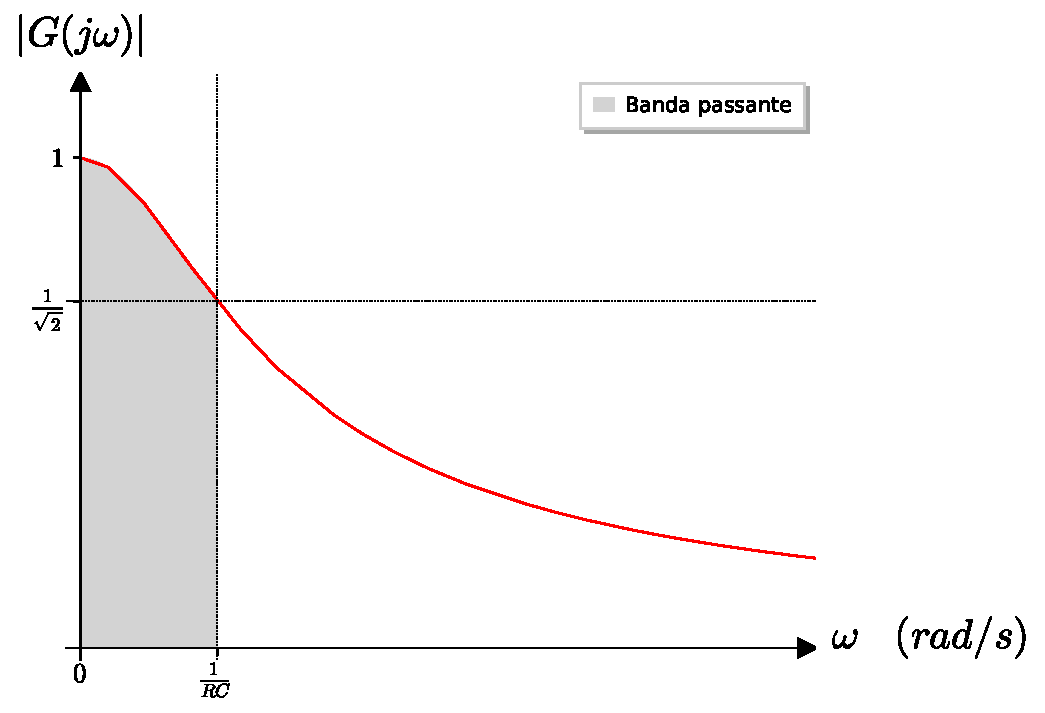
\includegraphics[width = \linewidth]{plot-0.pdf}
    \end{subfigure}%
    \begin{subfigure}{0.5 \linewidth}
      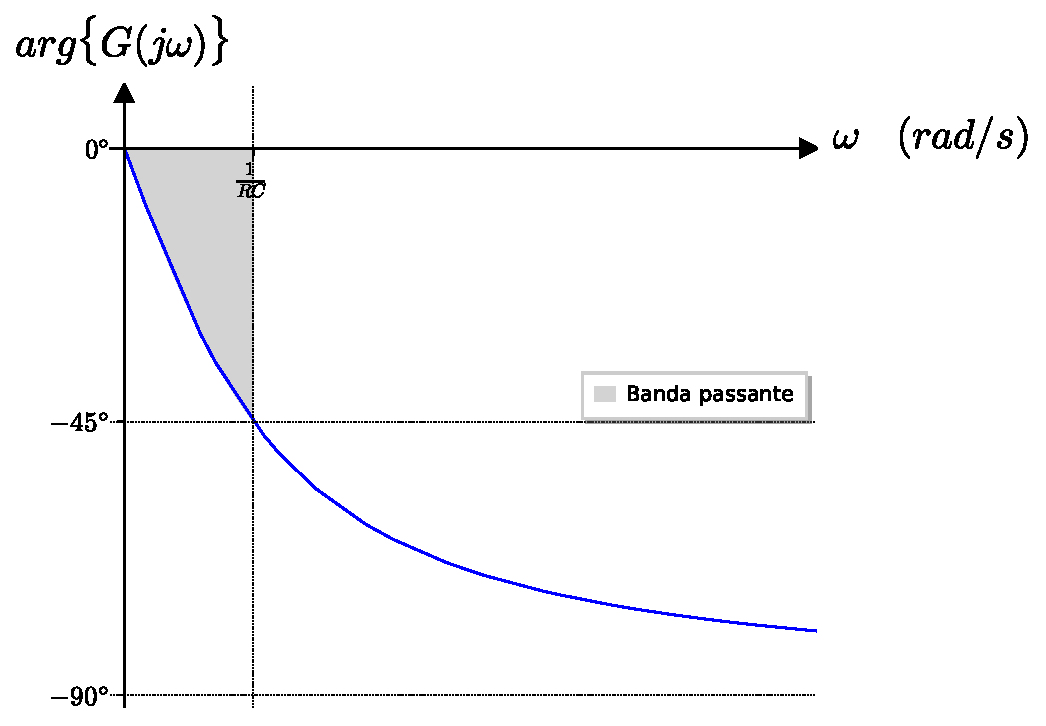
\includegraphics[width = \linewidth]{plot-1.pdf}
    \end{subfigure}
    \fontfigure{Elaboração Própria (\the\year)}
    \label{fig:grafico_passa_baixas}
  \end{figure}

  Outras características obtidas analisando o gráfico é que de fato ele se comporta como um filtro passa-baixas, já que o módulo da razão da tensão de saída pela de entrada, diminui drasticamente conforme se aumenta a frequência angular, em torno da frequência de corte.
  

  % Seção 3. Conclusão
  \section{Conclusão}
    \lipsum[2-3]
  % ---

  % --- Elementos pós-textuais (NBR 14724/2011) ---
  % ---
  \backtext%
  \bibliography{references} % Referências (obrigatório)
  %                           Glossário   (opcional)
  %                           Apêndice    (opcional)
  %                           Anexo       (opcional)
  %                           Índice      (opcional)
  % ---

\end{document}